% Ambipolar capacitance matrix C^amb as a fully-connected mesh (K5).
% One node per carrier, a capacitor between every pair. Each capacitor half is
% coloured by the species of its node (matching the ESBD species palette).
\documentclass[tikz, border=4pt]{standalone}
\usepackage[american]{circuitikz}
\usetikzlibrary{calc}

\definecolor{spA}{HTML}{377EB8} % electron
\definecolor{spB}{HTML}{E41A1C} % lithium
\definecolor{spC}{HTML}{80B030} % chloride
\definecolor{spD}{HTML}{8A4FA0} % oxide
\definecolor{spE}{HTML}{E6AB02} % silver

% Two-colour capacitor A--B: A's half in colour cA, B's half in cB. Renders the
% capacitor twice, each pass clipped to one side of the perpendicular bisector.
% Optional first arg = extra draw style (e.g. dashed).
\newcommand{\bicap}[5][]{% [style] A B cA cB
  \path (#2) -- (#3) coordinate[midway] (bcM);
  \begin{scope}
    \pgfinterruptboundingbox
    \clip let \p1=(#2), \p2=(#3), \n1={atan2(\y2-\y1,\x2-\x1)} in
      [rotate around={\n1:(bcM)}] ($(bcM)+(-6,-6)$) rectangle ($(bcM)+(0,6)$);
    \endpgfinterruptboundingbox
    \draw[#1,#4] (#2) to[C] (#3);
  \end{scope}
  \begin{scope}
    \pgfinterruptboundingbox
    \clip let \p1=(#2), \p2=(#3), \n1={atan2(\y2-\y1,\x2-\x1)} in
      [rotate around={\n1:(bcM)}] ($(bcM)+(0,-6)$) rectangle ($(bcM)+(6,6)$);
    \endpgfinterruptboundingbox
    \draw[#1,#5] (#2) to[C] (#3);
  \end{scope}
}

\begin{document}
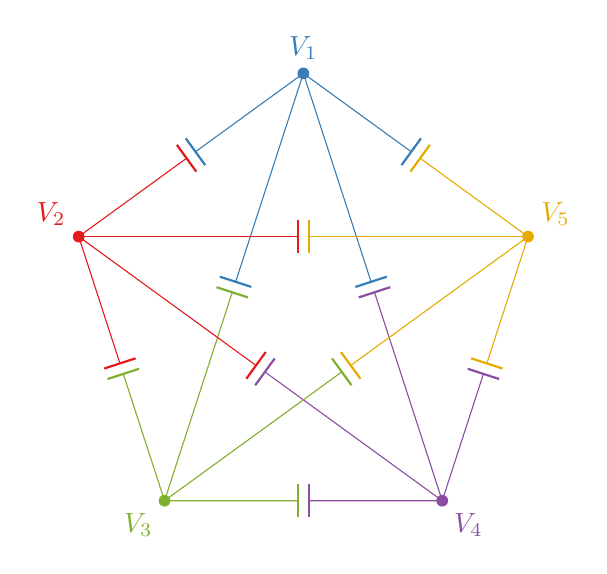
\begin{tikzpicture}
  \ctikzset{bipoles/length=0.7cm}

  % 5 carrier nodes on a pentagon, apex up, one species colour each
  \foreach \i/\c in {1/spA, 2/spB, 3/spC, 4/spD, 5/spE} {
    \coordinate (N\i) at ({72 * (\i - 1) + 90}: 3);
    \node[circle, fill=\c, inner sep=1.5pt,
          label={[label distance=-1pt, text=\c]{72 * (\i - 1) + 90}:$V_{\i}$}] at (N\i) {};
  }

  % a capacitor between every pair, each half coloured by its node
  \bicap{N1}{N2}{spA}{spB}
  \bicap{N1}{N3}{spA}{spC}
  \bicap{N1}{N4}{spA}{spD}
  \bicap{N1}{N5}{spA}{spE}
  \bicap{N2}{N3}{spB}{spC}
  \bicap{N2}{N4}{spB}{spD}
  \bicap{N2}{N5}{spB}{spE}
  \bicap{N3}{N4}{spC}{spD}
  \bicap{N3}{N5}{spC}{spE}
  \bicap{N4}{N5}{spD}{spE}
\end{tikzpicture}
\end{document}
